%%% Globale Einstellungen und Laden von Paketen (~Bibliotheken)
\documentclass[aspectratio=169,presentation]{beamer}
%\documentclass[aspectratio=169,handout]{beamer}

\usetheme{Boadilla} % Bestimmt das gesamte Erscheinungsbild, die folgenden fand ich grundsätzlich ganz passend:
% Hannover, Singapore, Malmoe, Boadilla, CambridgeUS

\useinnertheme{default}

% setting locales
\usepackage[utf8]{inputenc}
\usepackage[T1]{fontenc}
\usepackage[ngerman]{babel}
\usepackage{lmodern}
\usepackage[locale=DE,mode=math,list-final-separator={ oder },range-phrase={ bis },scientific-notation=false,group-digits=integer]{siunitx}

% package includes
\usepackage{tikz}
\usetikzlibrary{positioning,automata}
\usepackage{xcolor}
\usepackage{listings}

%listing setup
\definecolor{pblue}{rgb}{0.13,0.13,1}
\definecolor{pgreen}{rgb}{0,0.5,0}
\definecolor{pred}{rgb}{0.9,0,0}
\definecolor{pgrey}{rgb}{0.46,0.45,0.48}
\definecolor{javared}{rgb}{0.6,0,0} % for strings
\definecolor{javagreen}{rgb}{0.25,0.5,0.35} % comments
\definecolor{javapurple}{rgb}{0.5,0,0.35} % keywords
\definecolor{javadocblue}{rgb}{0.25,0.35,0.75} % javadoc

\lstset{language=c,
	basicstyle=\ttfamily,
	keywordstyle=\color{javapurple}\bfseries,
	stringstyle=\color{javared},
	commentstyle=\color{javagreen},
	morecomment=[s][\color{javadocblue}]{/**}{*/},
	tabsize=2,
	showspaces=false,
	showstringspaces=false
}


%%% (Wahrscheinlich ziemlich dreckige) Umsetzung von Spezialframes, die nur groß den Titel beinhalten
\newcommand{\sectionframe}[1]{
	\begin{frame}
		\vfill
		\Huge
		\centering
		\usebeamercolor[fg]{title}
		#1
		\vfill
		\par
	\end{frame}
}



%%% Zentrales Festelegen von Terminnummer und Datum
\newcommand{\terminNummer}{5}
\date{30. April 2019}
%%%



\begin{document}
\title[CE Tutorium]{Tutorium zu\\Computer-Engineering\\im SS19}
\subtitle{Termin \terminNummer}
\author[Otto]{Jakob Otto}
\institute{HAW Hamburg}
\subject{CE Tutorium}
\pgfdeclareimage[height=0.5cm]{university-logo}{logo-haw-2017}
\logo{\href{http://haw-hamburg.de}{\pgfuseimage{university-logo}}}

\titlepage

%---------------------------------------------------------------------------------------------------------------------
%	Ablauf
%---------------------------------------------------------------------------------------------------------------------
\section{Was steht an?}
\begin{frame}{Ablauf}
	\begin{columns}
		\column{0.6\textwidth}
		\begin{itemize}
			\item Praktikum
      \begin{itemize}
        \item Was ist ein Timer?
        \item Prescaler
        \item ARR/ARPE
			\end{itemize}
		\end{itemize}
		\column{0.4\textwidth}
		
\includegraphics[width=0.6\textwidth]{kratzen}
	\end{columns}
\end{frame}

%---------------------------------------------------------------------------------------------------------------------
%	Ideen für Aufgabe 1
%---------------------------------------------------------------------------------------------------------------------
% timer? was ist das?
% prescaler -> Was tut er?
% ARR 
% ARPE?!

\section{Timer}
\begin{frame} {Timer}
  \begin{itemize}
    \item eigentlich ein Counter
    \item zählt Ticks von internem Quarz/extern
    \item bei maximalem Zählstand kann zB IRQ ausgelöst werden 
    \begin{itemize}
      \item[$\rightarrow$] Timer startet dann von vorn
    \end{itemize}
  \end{itemize}
\end{frame}

\begin{frame}
  \begin{center}
    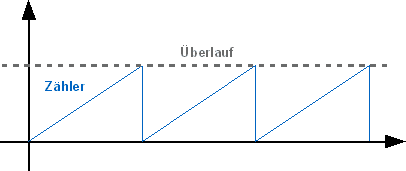
\includegraphics[width=.7\textwidth]{kurve_timer}  
  \end{center}
\end{frame}


\begin{frame}{Prescaler}
  \begin{itemize}
    \item Systemfrequenz meist zu hoch um Sinnvoll zu sein
    \begin{itemize}
      \item[$\rightarrow$] Wertebereich wird zu schnell verlassen
    \end{itemize} 
    \item dafür gibt es Prescaler
    \item weiterer Zähler, der eingehenden takt \glqq{}vorteilt\grqq{}
    \item Auflösung wird geringer
    \item Wertebereich wird seltener verlassen.
  \end{itemize}
\end{frame}

\begin{frame}{Aufbau Timer}
  \begin{center}
    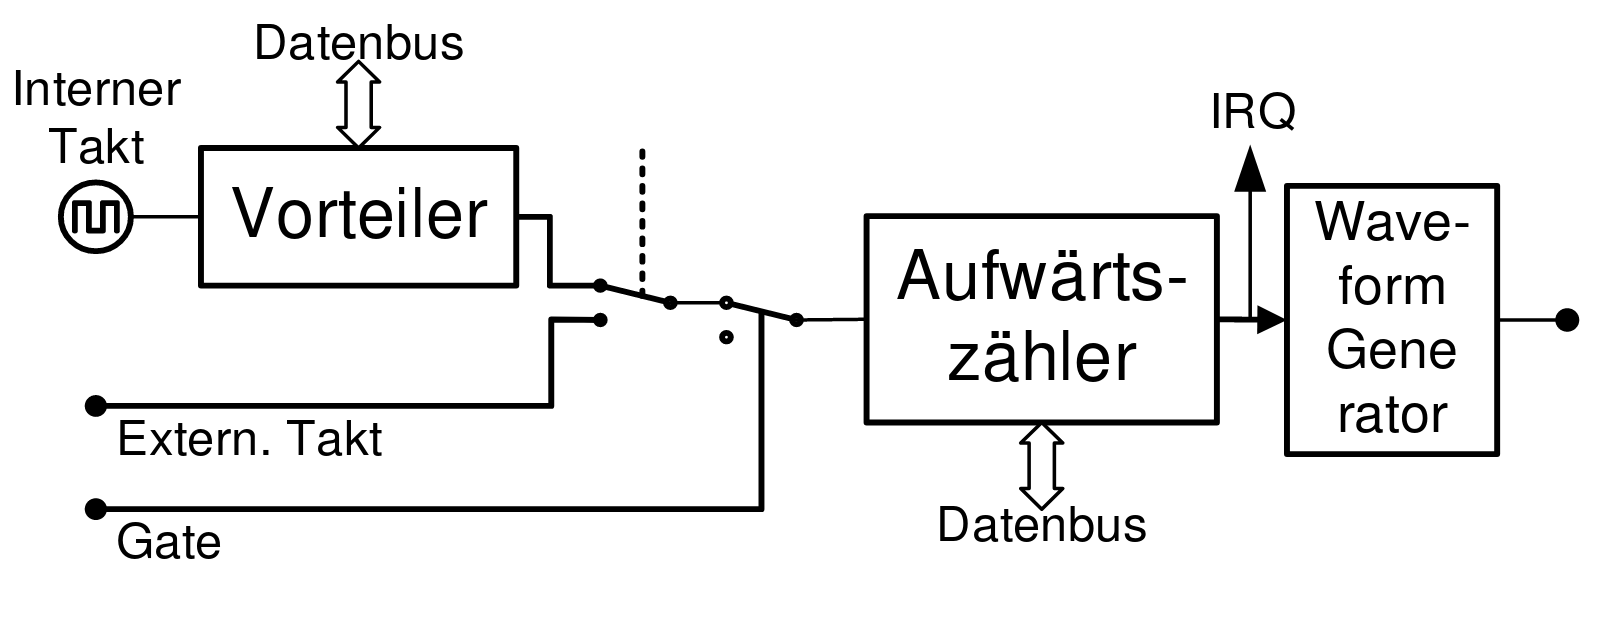
\includegraphics[width=\textwidth]{timer_generell}
  \end{center}
\end{frame}

\section{ARR}
\begin{frame}{ARR}
  \begin{itemize}
    \item Das ARR (AutoReloadRegister) beinhaltet einen eigenen Endwert.
    \item Zählstand wird mit dem Wert verglichen
    \item Bei erreichen:
    \begin{itemize}
      \item reset vom Zählstand
      \item prescaler $\rightarrow$ tick an timer
      \item Timer $\rightarrow$ IRQ
    \end{itemize}
  \end{itemize}
\end{frame}

\begin{frame}{ARR}
  \begin{center}
    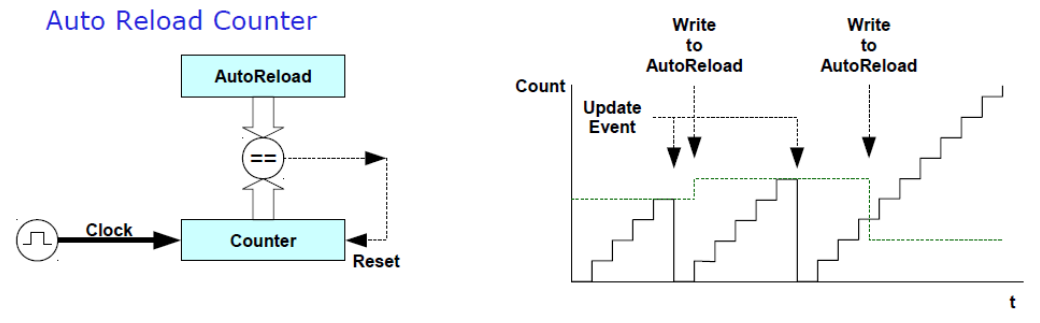
\includegraphics[width=\textwidth]{ARPE_disable}    
  \end{center}
\end{frame}

\section{ARPE}
\begin{frame}{ARPE}
  \begin{itemize}
    \item ARR kann zur laufzeit verändert werden
    \item Timer kann schon über den neuen Wert gezählt haben
    \begin{itemize}
      \item[$\rightarrow$] zählt dann bis maxwert des Registers
    \end{itemize}
    \item um das zu vermeiden gibts das ARPE-bit
    \item änderung wird durch shadow-register verzögert
    \begin{itemize}
      \item[$\rightarrow$] erst bei nächstem overflow ins ARR übernommen
    \end{itemize}
  \end{itemize}
\end{frame}

\begin{frame}{ARPE}
  \begin{center}
    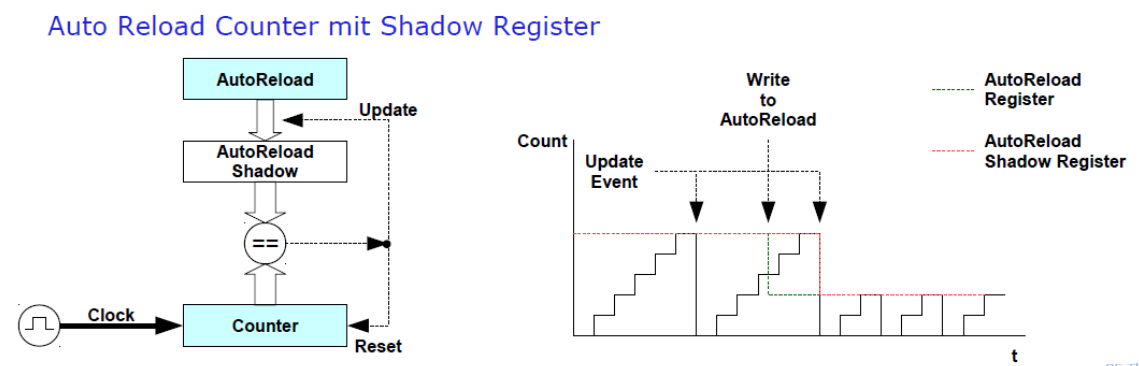
\includegraphics[width=\textwidth]{ARPE_enable}    
  \end{center}
\end{frame}

\begin{frame}[fragile]{Code}
  \begin{lstlisting}
//Timer setup
TIM1->CR1 = 0; // disable timer1
TIM1->CR2 = 0; // disable timer2
TIM1->PSC = 0; // prescaler value
TIM1->ARR = (SYS_FREQ / TIMER_FREQ) -1; // 
TIM1->DIER = TIM_DIER_UIE; // enable Interrupt
TIM1->CR1 = TIM_CR1_ARPE; // Auto Reload preload enable

// enable timer
TIM1->CR1 |= TIM_CR1_CEN;
  \end{lstlisting}
\end{frame}

\sectionframe{\href{https://www.st.com/content/ccc/resource/technical/document/application_note/group0/91/01/84/3f/7c/67/41/3f/DM00236305/files/DM00236305.pdf/jcr:content/translations/en.DM00236305.pdf}{General-purpose timer cookbook}}

\end{document}